%% heading for this chapter
This chapter outlines and highlights useful background that will be explored in further detail in upcoming chapters as well as provides an outline for the. 
Notably this section introduces and summarizes the relationships between the search for physics beyond the standard model (BSM), DUNE, and novel pixel-based detectors. 
We begin with an introduction on the standard model, and how both its success and short comings drive larger and more expensive detectors at the intensity frontier.
Next, we become more specific and discuss DUNE which is an example of a new, large, and expensive detector which aims to push beyond the Standard Model.
Afterwards we elaborate on the type of detector, which DUNE is based: Time Projection Chambers (TPCs).
Finally, we relate the work presented in this dissertation is based on TPCs and how the novel readout design used here is suited for future expansion into larger detectors.
We follow this pattern of beginning large and becoming small because that's how we also build detectors: we begin with the large and travel towards the small.

%% BSM
\section{Looking for exceptions to the Standard Model}

In the history of science, it is easily argued that the most successful of all models has been the Standard Model of physics. 
Yet, despite its numerous achievements in predictive power and experimental verification we know today that it has crucial shortcomings. 
The Standard Model (SM) has no ability to account for Dark Matter or Dark Energy in the universe, nor the distribution (or the hierarchy) of neutrino masses, nor is it able to relate how gravity interacts with the other fundamental forces of nature (Unification).
These short-comings offer hints to search for physics at different frontiers of physics.

%% a brief shoutout to the different frontier of a high energy physics here, and discuss specifically the intensity
The Intensity Frontier of Physics (\citep{intensityfrontier2012_Hewett}) is one which requires very large and very precise measurements to gain the statistics to declare an observation. 


We briefly discuss some short-comings of the Standard Model today, and elaborate the current status of the searches.

Large Scale detectors hunting for New Physics (NP) have continued to grow in size, energy sensitivity, and importantly cost: \citep{Juno:2022103927}.


\subsection{Where is the Hadron Decay}
%% what is the princpal of hadron decay, put thta interaction here


% ignore dark matter for now
%\subsection{Shining light on the Dark Sector}
%% dark energy and dark matter
%% Jeff / Jack / Thorne

\subsection{The Neutrino Hunt}
%% neutrino oscillation measurement here

%% solar neutrinos

%% neutrino mass oscillations

%% what are the problems of neutrinos and which ones do we care about (electron / muon from a beam)
Super-K / SNO / KamLand / NOvA / daya bay / RENO / double chooz / t2k / minos

\citep{SNO_2002_neutrino_PhysRevLett.89.011301, neutrino_measurement_NOvA_2019_prl, t2k_2011_neutrino_PhysRevLett.107.041801}
\cite{reno_2012_neutrino_PhysRevLett.108.191802}
%\cite{minos_2006_neutrino_PhysRevLett.97.191801}
\citep{FUKUDA2002_solar_neutrino_oscillation}
\citep{kamland_2003_neutrino_PhysRevLett.90.021802}
\citep{daya_bay_2012_neutrino_PhysRevLett.108.171803}
\citep{doubleChooz_2012_neutrino_PhysRevLett.108.131801}

% Double Chooz used two identical gadolinium-doped liquid scintillator detectors
% t2k is (Tokai to Kamioka) is a long-baseline neutrino experiment, over 295 km
%% nd is at j-parc, far detector is at superk


%% physical interaction of neutrino scattering here


%% Motivating Source of TPCs
\section{Time Projection Chambers}

Time Projection Chambers (\citep{lartpc:nygren}) have been shown to be extremely useful in high energy physics experiments due, in part, to their high resolution in both timing and spatial dimensions.


\subsection{Noble Gases and Time Projection Chambers}

The technology of TPCs has greatly matured since their original inception. 
As a result, the technical applications of TPCs are far reaching and find practical uses
in many kinds of detectors across HEP. TPCs can also incorporate two phases of a substance (liquid and gas), called Dual Phase (DP) TPCs.

the Xenon-1T is a dark matter experiment which is a dual-phase TPC \citep{Aprile_2017_xenon1T}.

The LUX experiment is a single phase TPC also hunting for dark matter.


A specific kind of TCP is a Liquid Argon Time Projection Chamber (LArTPC) \citep{rubbia1977liquid}.

%% include relevant LArTPCs here
recent work on LArTPCs (\citep{ArgoNeuT:PhysRevD.99.012002}, \citep{MicroBooNE:Acciarri_2017}, \citep{LArIAT:Acciarri_2020}).


Energy resolution of the LArTPCs within DUNE are still unknown to within a factor of 4 \citep{lartpc_energy_resolution:PhysRevD.99.036009}.


%% Highlight what DUNE is and its purpose
\section{The Deep Underground Neutrino Experiment}

The Deep Underground Neutrino Experiment (DUNE) is a long-baseline neutrino beam experiment \cite{DUNE_TDR_V1_Abi_2020, DUNE_FD_TDRv2_2020, DUNE_TDRv3_Abi_2020, DUNE-FD_TDRv4:Abi_2020}. 
DUNE is composed two detectors, a near (ND) and a far (FD) which are separated by a distance of 1300 km. 
The ND is located at Fermilab and its purpose is to characterize the source neutrino beam created there.
The FD is composed of four separate 10 kiloton modules, all of which will be a single-phase (SP) LArTPC based detector.
Two of these four modules at least will use a known wire-based readout technology and a vertical drift-readout.
The two remaining modules are considered modules of opportunity and their readout technology is yet unknown.
A purpose of this dissertation is show the viability of a novel readout technology.

\begin{figure}[ht!]
\centering
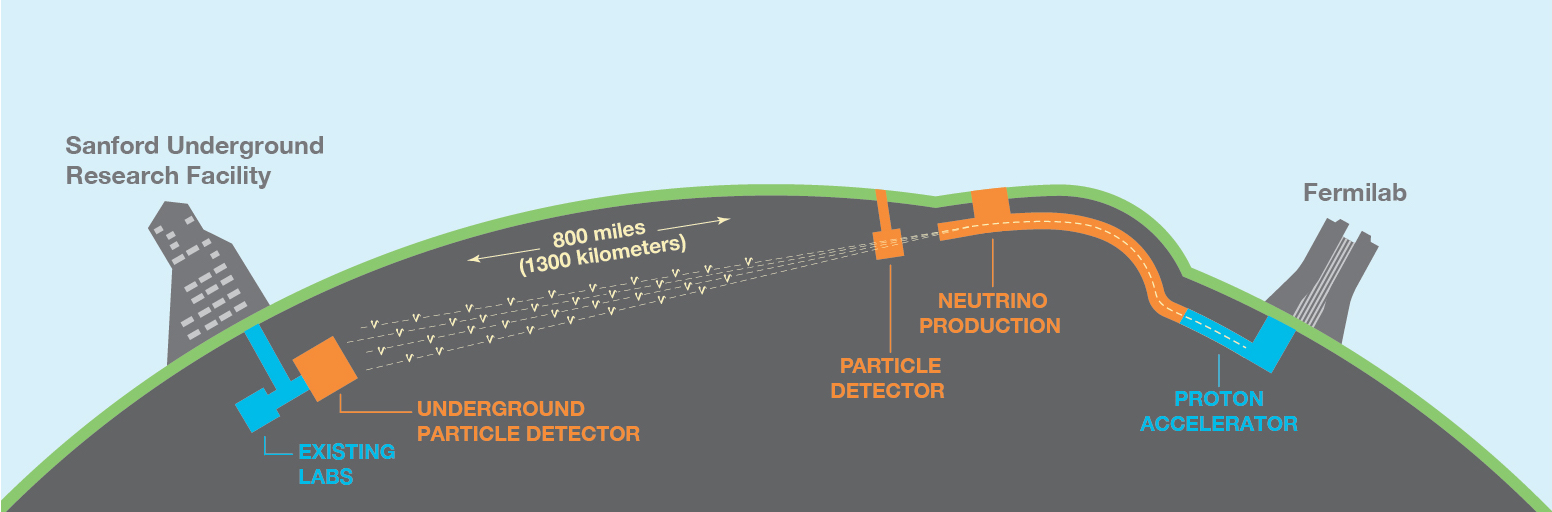
\includegraphics[width=\textwidth]{images/LBNE_Graphic_061615_2016.jpg}
\caption{Simple Draw up of DUNE FD taken from \citep{dune_cdr_2016_arxiv}}
\end{figure}

DUNE has three main science goals, all of which are geared towards pushing beyond the standard model:
\begin{itemize}
    \item Hadron Decay
    \item Neutrinos from Core-collapse supernovae
    \item Beamline neutrino interactions.
\end{itemize}

We will discuss the relevance of each of these items, and in \ref{chap:qpix} we will further discuss how the work presented here relates to each of these topics. 


Conventional horizontal drift detection for foreseeable DUNE modules are already considered possible for lengths up to 6.5m \citep{DUNE_Vertical:Paulucci_2022}.


\subsection{Hadron Decay}
\label{sect:intro_decay}

Second generation proton decay studies in the ICARUS experiment: \citep{ICARUS_2001}.

%% why do we care about hadron decay

\subsection{Supernova Studies}
\label{sect:intro_supernova}

%% why do we care about supernova neutrinos, what will they tell us?
The principal decay chain follows the pattern:
\begin{equation}
    \nu_{e} + ^{40}Ar \rightarrow e^- + ^{40}Kr^*
\end{equation}

%% text from the cdr 
% The neutrinos from a core-collapse supernova are emitted in a burst of a few tens of seconds
% duration, with about half the signal emitted in the first second. The neutrino energies are mostly
% 4The lifetime shown here is divided by the branching fraction for this decay mode, $\tau$ /B, and as such is a partial
% lifetime.
% Volume 1: The LBNF and DUNE Projects LBNF/DUNE Conceptual Design Report
% Chapter 2: DUNE Science 2–18
% in the range 5–50 MeV, and the luminosity is divided roughly equally between the three known
% neutrino flavors. Current experiments are sensitive primarily to electron antineutrinos ($\nu_e$), with
% detection through the inverse-beta decay process on free protons5
% , which dominates the interaction
%rate in water and liquid-scintillator detectors. Liquid argon has a unique sensitivity to the electronneutrino (νe) component of the flux, via the absorption interaction on 40Ar,

% This interaction can be tagged via the coincidence of the emitted electron and the accompanying
% photon cascade from the 40K∗ de-excitation. About 3000 events would be expected in a 40−kt
% fiducial mass liquid argon detector for a supernova at a distance of 10 kpc. In the neutrino channel
% the oscillation features are in general more pronounced, since the νe spectrum is always significantly
%different from the νµ (ντ ) spectrum in the initial core-collapse stages, to a larger degree than is
%the case for the corresponding ν¯e spectrum. Detection of a large neutrino signal in DUNE would
% help provide critical information on key astrophysical phenomena such as
%  the neutronization burst,
%  formation of a black hole,
%  shock wave effects,
%  shock instability oscillations, and
%  turbulence effects.
% In addition to yielding unprecedented information on the mechanics of the supernova explosion,
% the observation of a core-collapse supernova in DUNE will also probe particle physics, providing
% neutrino oscillation signatures (with sensitivity to mass hierarchy and “collective effects” due to
% neutrino-neutrino interactions), as well as tests for new physics such as Goldstone bosons (e.g.,
% Majorons), neutrino magnetic moments, new gauge bosons (“dark photons”), “unparticles” and
% extra-dimensional gauge bosons

\subsection{Neutrino Beam Studies}

%% why do we care about neutrino beam oscillations

%% what is the difference between NC and CC neutrino interactions.

\section{Pixelated Detectors in the Current Century}

Finally, in this last section we discuss recent progress of various detector technologies moving towards pixelization.
There are many motivating pressures for new detectors to adopt pixelated designs. 
Below we discuss two contributing factors: the development of electronics and computing algorithms.

First, previously pixelated detectors have historically been more difficult because of the issues of cost and size regarding the number of readout channels.
This is being addressed, in part, by the advent of newer, cheaper, and larger Field-Programmable-Gate Arrays (FPGAs).
One method for reducing the electronic overhead required in pixelated detectors is to use digital multiplexing.
Cheap, high channel FPGAs directly solve this problem. 
Other electronics development, such as the Silicon-Photomultiplier, offer much cheaper alternatives for large pixel counters compared to their historical counter-parts. 

%% antihydrogen
\citep{Sadowski_2017}
Another driving factor is the the development of Machine Learning (ML) algorithms, particularly Convectional Neural Network (CNN \citep{Sadowski2017DeepLI}). 
Recent industry has driven the need for CNNs to be able to correctly identify and label 2-D images of various kinds, and thus championed much of progress in this field and spawned many kinds of CNN algorithms. 
%% cite sadowski here
Recently, it has been shown how these kinds of algorithms extend into High Energy Physics (HEP) for particle identification.
A major issue at the Intensity Frontier of physics is the sheer amount of data to store and process. 
These ML algorithms provied a developed tool to automate the analysis of huge amounts of data ($>> 1 TB$) and have been shown to be quite accurate ($>99\%$) at particle identification in LArTPCs.

%% LArPix / Argon Cube
\subsection{Current Pixelization Efforts in TPCs}


%% goeldi inspiration here from LArPix

Additional work has been performed in recent years which show that LArTPCs can also utilized a pixel-based readout \citep{larpix:Dwyer_2018}, \citep{Asaadi_2018}.

%% SVSC
\subsection{Comments on Other applications of Pixelization}

\subsubsection{SANDD}

Another Example of a pixelated detector is \citep{SUTANTO2021_sandd_165409}.


\subsubsection{The Single Volume Scatter Camera}

This work is presented in greater detail in (Appendicies-\ref{chap:OS1}/\ref{chap:OS2}) and represents a substantial amount of my own individual contribution. 
I am the 2nd author on the the paper described in Appendix-\ref{chap:OS1} and the corresponding author of Appendix-\ref{chap:OS2}, where I also collected and analyzed all presented data therein.